% Modified Template by Jonathan Doucette and Kevin Multani, original by: Jonathan Ward

\documentclass[12pt]{article} 
\usepackage[english]{babel}
\usepackage[utf8]{inputenc}
\usepackage{amsmath} % AMS Math Package
\usepackage{amsthm} % Theorem Formatting
\usepackage{amssymb} % Math symbols such as \mathbb
\usepackage{graphicx} % Allows for eps images
\usepackage{multicol} % Allows for multiple columns
\usepackage[dvips,letterpaper,margin=1in,bottom=1in]{geometry}
\usepackage{hyperref}
\usepackage{parskip} % Removes indentation from paragraphs
\usepackage{xcolor,xspace,soul} % Colour, spacing, and highlighting
\usepackage{mathrsfs}
\usepackage{bm} % For bold math symbols
\usepackage{amscd}
\usepackage[all,cmtip]{xy}
%\usepackage{bbm}
\usepackage{titling}
\usepackage{listing} % for code snippets
%\usepackage{minted} % for code snippets
\usepackage{enumerate}
\usepackage{fancyhdr}
\usepackage[]{physics}
\usepackage[makeroom]{cancel}
\usepackage{pdfpages}
\usepackage[]{mcode}
\usepackage[title]{appendix}

% ***********************************************************
% ********************** BEGIN TITLE PAGE *******************
% ***********************************************************
\newcommand*{\titleGM}{\begingroup % Create the command for including the title page in the document
\hbox{ % Horizontal box
\hspace*{0.2\textwidth} % Whitespace to the left of the title page
\rule{1pt}{\textheight} % Vertical line
\hspace*{0.05\textwidth} % Whitespace between the vertical line and title page text
\parbox[b]{0.75\textwidth}{ % Paragraph box which restricts text to less than the width of the page

{\noindent\Huge\bfseries MATH 521}\\[2\baselineskip] % Title
{\large \textit{Assignment 4}}\\[4\baselineskip]
%{\large \textsc{ Jonathan Doucette }} % Author name

\vspace{0.5\textheight} % Whitespace between the title block and the publisher
{\noindent \today }\\[\baselineskip]
%{\noindent Student Number: 35298124 }\\[\baselineskip] 
%{\noindent \footnotesize All problems below are \textit{Copyright \copyright \space 2018 Timm Treskatis. All Rights Reserved.} }\\[\baselineskip]
} % end parbox
} % end hbox
\endgroup}

 % Sets margins and page size
\pagestyle{fancy} 

%\lhead{Jonathan Doucette}
\rhead{\today}
\rfoot{Page \thepage}
\cfoot{}

\makeatletter % Need for anything that contains an @ command 
\renewcommand{\maketitle} % Redefine maketitle to conserve space
{ \begingroup \vskip 10pt \begin{center} \Huge {\bf \@title}
\vskip 10pt \large \@author \hskip 20pt \@date \end{center}
  \vskip 10pt \endgroup \setcounter{footnote}{0} }
\makeatother % End of region containing @ commands

% ***********************************************************
% ********************** END TITLE PAGE *********************
% ***********************************************************

% ***********************************************************
% ********************** BEGIN NEW COMMANDS *****************
% ***********************************************************

\renewcommand{\labelenumi}{(\alph{enumi})} % Use letters for enumerate
\let\vaccent=\v % rename builtin command \v{} to \vaccent{}

%% MISC
\newcommand{\ab}[1]{\left| #1 \right|} % for absolute value
\newcommand{\avg}[1]{\left< #1 \right>} % for average
\let\underdot=\d % rename builtin command \d{} to \underdot{}
\let\baraccent=\= % rename builtin command \= to \baraccent
\renewcommand{\=}[1]{\stackrel{#1}{=}} % for putting numbers above =
\providecommand{\fr}{\frac}
\providecommand{\RR}{\mathbb{R}}
\providecommand{\CC}{\mathbb{C}}
\providecommand{\NN}{\mathbb{N}}
\providecommand{\e}{\epsilon}
\DeclareMathOperator{\di}{d\!}
\newcommand*\ieval[3]{\left.#1\right\rvert_{#2}^{#3}}

%% Vectors
\renewcommand{\v}[1]{\ensuremath{\mathbf{#1}}} 
\newcommand{\gv}[1]{\ensuremath{\mbox{\boldmath$ #1 $}}} % for vectors of Greek letters
\newcommand{\uv}[1]{\ensuremath{\mathbf{\hat{#1}}}} % for unit vector
\providecommand{\wave}[1]{\v{\tilde{#1}}}

%% DERIVATIVES
\renewcommand{\d}[2]{\frac{d #1}{d #2}} % for derivatives
\newcommand{\dubd}[2]{\frac{d^2 #1}{d #2^2}} % for double derivatives
\newcommand{\pd}[2]{\frac{\partial #1}{\partial #2}} % for partial derivatives
\newcommand{\pdd}[2]{\frac{\partial^2 #1}{\partial #2^2}} % for double partial derivatives

%% Operators
\newcommand{\Gradient}{\ensuremath{\mbox{\boldmath$\nabla$}}} % gradient

%% Text
\newcommand{\mathcolorbox}[2]{\colorbox{#1}{$\displaystyle #2$}}
\newcommand{\hlfancy}[3]{\textcolor{#1}{\sethlcolor{#2}\hl{#3}}}
\newcommand{\TODO}[1]{\hlfancy{red}{yellow}{\textbf{TODO: #1}}}

%% Code
%\newcommand{\code}[1]{\mintinline{C}{#1}}
%\newcommand{\code}[1]{\texttt{#1}}
\newcommand{\code}[1]{\lstinline[columns=fixed]{#1}}
\newcommand{\includecode}[1]{\lstinputlisting{#1}}

% ***********************************************************
% ********************** END NEW COMMANDS *******************
% ***********************************************************

% ***********************************************************
% ********************** BEGIN NEW ENVS *********************
% ***********************************************************

% Theorem
\newenvironment{theorem}[2][Theorem]{\begin{trivlist}
\item[\hskip \labelsep {\bfseries #1}\hskip \labelsep {\bfseries #2.}]}{\end{trivlist}}
% Lemma
\newenvironment{lemma}[2][Lemma]{\begin{trivlist}
\item[\hskip \labelsep {\bfseries #1}\hskip \labelsep {\bfseries #2.}]}{\end{trivlist}}
% Corollary
\newenvironment{corollary}[2][Corollary]{\begin{trivlist}
\item[\hskip \labelsep {\bfseries #1}\hskip \labelsep {\bfseries #2.}]}{\end{trivlist}}

% Exercise
\newenvironment{exercise}[2][Exercise]{\begin{trivlist}
\item[\hskip \labelsep {\bfseries #1}\hskip \labelsep {\bfseries #2.}]}{\end{trivlist}}
% Problem
\newenvironment{problem}[2][Problem]{\begin{trivlist}
\item[\hskip \labelsep {\bfseries #1}\hskip \labelsep {\bfseries #2.}]}{\end{trivlist}}
% Question
\newenvironment{question}[2][Question]{\begin{trivlist}
\item[\hskip \labelsep {\bfseries #1}\hskip \labelsep {\bfseries #2.}]}{\end{trivlist}}
% Solution
\newenvironment{solution}{\begin{proof}[Solution]}{\end{proof}}

% Afterword
\newenvironment{afterword}[2][Appendix]{\begin{trivlist}
\item[\hskip \labelsep {\bfseries #1}\hskip \labelsep {\bfseries #2}]}{\end{trivlist}}

% ***********************************************************
% ********************** END NEW ENVS ***********************
% ***********************************************************

% ***********************************************************
% ********************** END TITLEPAGE **********************
% ***********************************************************

%\documentclass[10pt,letterpaper]{scrartcl}
%\usepackage{amsfonts,amsmath,amssymb,braket,xcolor,dsfont,enumerate,fontawesome,graphicx}
\usepackage{amsfonts,amsmath,amssymb,braket,xcolor,enumerate,graphicx}
\usepackage[hidelinks]{hyperref}
\usepackage{listings,multicol,mathtools,textcomp,tikz,pgfplots,wrapfig}
%\usepackage[inner=2cm,outer=2cm,top=2cm,bottom=2cm]{geometry}
\usepackage{tabularx}
\usepackage{booktabs}
\usetikzlibrary{arrows}
%\pgfplotsset{compat=1.12}

\pagestyle{empty}
\setlength{\parindent}{0pt}
\setlength{\parskip}{6pt}

%\newcommand{\dx}{\;\mathrm{d}x}

\begin{document}

\begin{minipage}{.2\textwidth}

\includegraphics[width=42pt]{ubc-logo.png}
\end{minipage}
\hfill
\begin{minipage}{.75\textwidth}
\setlength{\parskip}{6pt}
\begin{flushright}
{\sffamily
\textbf{MATH521}\\
\textbf{Numerical Analysis of Partial Differential Equations}

Winter 2017/18, Term 2\\
Timm Treskatis
}
\end{flushright}
\end{minipage}

\section*{Homework Assignment 10}

Please submit the following files as indicated below: %\hfill \faFileCodeO \: source code \hfill \faFilePdfO \: PDF file \hfill \faFilePictureO \: image file \hfill \faFileMovieO \: video file

\paragraph*{Question 1 $\vert$ 2 marks}% $\vert$ \faFilePdfO}

On the assignment page you can find videos of four animated solutions of the parabolic problem
\begin{equation}\tag{H}\label{eq:heat}
\begin{aligned}
\partial_t u(t) - a \Delta u(t) &= f(t) && \text{in } Q = ]0,T[ \times \Omega\\
u(0) &= u_0 && \text{in } \Omega\\
\frac{\partial u}{\partial n} &= 0 && \text{on } \Sigma = ]0,T[ \times \partial \Omega
\end{aligned}
\end{equation}
with the data from Assignment 9. However, the initial condition has been replaced with the function
\begin{equation*}
u_0(x) =
\begin{dcases*}
50 & if $\lvert x - (1,1)^\top \rvert < 0.5$\\
20 & elsewhere
\end{dcases*}
\end{equation*}

Explain your observations.

% ------------------------------------------------------------ %
% Q1: Solution
% ------------------------------------------------------------ %
\vspace{0.5cm}
\begin{solution}
First, we note that since our initial condition in Assignment 9 was $u_0 = 20$ in $\Omega$, the only change in the initial condition is that now $u_0 = 20$ throughout $\Omega$, except for those points contained in the region $\lvert x - (1,1)^\top \rvert < 0.5$ wherein $u_0 = 50$.

Now, some initial observations:
\begin{itemize}
\item Our initial data has a discontinuous ``hot spot'' in the north-eastern corner of the domain.
\item The forcing term applies gaussianly distributed heat centred about the south-western corner of the domain for the first second of the five second simulation.
\item The heat equation will smooth out the discontinuity immediately in the continuous case due to the sharp discontinuity containing high frequency eigenmodes which are damped exponentially fast.
Ideal numerical schemes should mimic this effect.
\item Failure of the numerical scheme in handling the discontinuity effectively will likely lead to ringing of the solution, possibly with extreme ``wiggles'' and other effects due to instabilities.
\end{itemize}

And, additionally, some notes on the three methods used for solving the wave equation:
\begin{itemize}
\item The Crank-Nicolson method is only A-stable, and not strictly or strongly A-stable. In fact, in the limit as the frequency of the eigenmode goes to infinity, the eigenmode is not damped at all.
\item The backward Euler method is strongly A-stable, and in fact L-stable. This means that high frequency modes are damped immediately.
\item The $\theta$-method is strongly A-stable for $\theta > 1/2$. Like the backward Euler method, this means that high frequency modes will be exponentially damped, though since the $\theta$-method is not L-stable, they likely will not be damped as quickly.
\end{itemize}

\newpage
\paragraph*{Crank-Nicolson (\textsc{cn-50.webm}): $h=1/50$}
In finite elements simulations using linear finite elements, discontinuities cannot be represented exactly, and in particular discontinous functions will be approximated by continuous piecewise linear functions.
If the step size $h$ is large enough, the discontinuity will actually not be all that discontinuous in the discrete approximation.
As can be seen from the video, the high-frequency modes of the initial condition which theoretically should not be smoothed out my the Crank-Nicolson method do manage to smooth out as time moves on.
This is likely due to the relative large spatial resolution.
It should be noted, however, that this process does not at all happen quickly, and there is noticeable numerical ringing around the ``discontinuity''.

\paragraph*{Crank-Nicolson (\textsc{cn-200.webm}): $h=1/200$}
In contrast with the Crank-Nicolson solution with $h=1/50$ above, here the discontinuous initial is indeed approximated well enough to show large amounts of ringing and instability near the region of discontinuity.
The discontinuity is in fact never smoothed out, as would be expected for the Crank-Nicolson method with discontinuous initial data.

\paragraph*{Backward Euler (\textsc{be-200.webm}): $h=1/200$}
The backward Euler method, being L-stable, immediately damps out the discontinuity in the initial condition.
The solution smooths out quickly and uniformly, and remains as such throughout the simulation.
In fact, the disconinuity appears to be smoothed out on the very first frame, as far as I can tell, and this should be expected for an L-stable method.

\paragraph*{The $\theta$-Method (\textsc{th-200.webm}): $\theta = 0.55,\,h=1/200$}
The $\theta$-method is strongly A-stable, and so the high-frequency discontinuity is damped out exponentially fast at the beginning of the simulation, and the temperature distribution is smooth throughout the domain.
As expected, however, the rate at which the damping occurs is slower than that of the backward Euler method, in which the smoothing occurs effectively immediately.


\end{solution}

\newpage

\paragraph*{Question 2 $\vert$ 1 mark}% $\vert$ \faFilePdfO}

We have seen that the homogeneous wave equation
\begin{equation}\tag{W}\label{eq:wave}
\begin{aligned}
\partial_t^2 u - c^2 \Delta u &= 0 && \text{in } Q = \left] 0,T\right[ \times \Omega\\
u(0) &= u_0 && \text{in } \Omega\\
\partial_t u(0) &= v_0 && \text{in } \Omega\\
u &= 0 && \text{on } \Sigma = ]0,T[ \times \partial \Omega
\end{aligned}
\end{equation}
with propagation speed $c>0$ can equivalently be re-written as
\begin{equation}\tag{W'}\label{eq:waveSystem}
\begin{aligned}
\partial_t u - v &= 0 && \text{in } Q = \left] 0,T\right[ \times \Omega\\
\partial_t v - c^2 \Delta u &= 0 && \text{in } Q = \left] 0,T\right[ \times \Omega\\
u(0) &= u_0 && \text{in } \Omega\\
v(0) &= v_0 && \text{in } \Omega\\
u &= 0 && \text{on } \Sigma = ]0,T[ \times \partial \Omega\\
v &= 0 && \text{on } \Sigma = ]0,T[ \times \partial \Omega.
\end{aligned}
\end{equation}
Discretising with the $\theta$-method in time and linear finite elements in space leads to the coupled system for the vectors of nodal values $\vec{u}^h_+$ and $\vec{v}^h_+$
\begin{align*}
M^h \vec{u}^h_+ - \theta \Delta t M^h \vec{v}^h_+ &= M^h \vec{u}^h_\circ + (1-\theta) \Delta t M^h\vec{v}^h_\circ\\
\theta \Delta t c^2 K^h \vec{u}^h_+ + M^h \vec{v}^h_+ &= -(1-\theta) \Delta t c^2 K^h \vec{u}^h_\circ + M^h \vec{v}^h_\circ
\end{align*}
which has to be solved at every time step. Show that this is equivalent to the two smaller, successively solvable problems
\begin{align*}
\left(M^h + \left(\theta \Delta t c\right)^2 K^h\right) \vec{u}^h_+ &= M^h \left( \vec{u}^h_\circ + \Delta t \vec{v}^h_\circ\right) - \left( \theta\left(1-\theta\right) \left(\Delta t c\right)^2 \right)K^h \vec{u}^h_\circ\\
M^h \vec{v}^h_+ &= M^h \vec{v}^h_\circ - \Delta t c^2 K^h \left( \theta \vec{u}^h_+ + \left(1-\theta\right) \vec{u}^h_\circ\right).
\end{align*}


% ------------------------------------------------------------ %
% Q1: Solution
% ------------------------------------------------------------ %
\vspace{0.5cm}
\begin{solution}
If we multiply the second equation of the coupled system by $\theta \Delta t$ and add it to the first equation of the coupled system and simply, we get
\begin{align}\label{eqn:uncoupled1}
\left(M^h + \left(\theta \Delta t c\right)^2 K^h\right) \vec{u}^h_+
&= M^h \left( \vec{u}^h_\circ + \Delta t \vec{v}^h_\circ\right) +
\left( \theta^2 \left(\Delta t c\right)^2  - \theta \left(\Delta t c\right)^2 \right)K^h \vec{u}^h_\circ\nonumber\\
&= M^h \left( \vec{u}^h_\circ + \Delta t \vec{v}^h_\circ\right) - \left( \theta\left(1-\theta\right) \left(\Delta t c\right)^2 \right)K^h \vec{u}^h_\circ,
\end{align}
which is the first desired equation of the new uncoupled system.

Now, if we simply subtract $\theta \Delta t c^2 K^h \vec{u}^h_+$ from both sides of the second equation of the coupled system and simply, we get 
\begin{align}\label{eqn:uncoupled2}
M^h \vec{v}^h_+
&= M^h \vec{v}^h_\circ + \left( \Delta t c^2 K^h \theta - \Delta t c^2 K^h \right) \vec{u}^h_\circ -
\left( \theta \Delta t c^2 K^h \right) \vec{u}^h_+ \nonumber \\
&= M^h \vec{v}^h_\circ - 
\Delta t c^2 K^h \left( \theta \vec{u}^h_+ + (1-\theta) \vec{u}^h_\circ \right),
\end{align}
which is the second desired equation of the new uncoupled system.

\end{solution}


\newpage

\paragraph*{Question 3 $\vert$ 2 marks}

\begin{enumerate}[(a)]
\item %\faFileCodeO \:
Download and complete the \textsf{FEniCS} script \texttt{hw10.py} to solve Problem \eqref{eq:wave} with the data provided.
\item %\faFilePdfO \: \faFilePictureO \:
Solve the wave equation
\begin{itemize}
\item with the (symplectic) implicit midpoint rule
\item with the backward \textsc{Euler} method
\item with the forward \textsc{Euler} method
\end{itemize}
and look at the solutions in \textsf{ParaView}.

\emph{Hint:} Use the `Warp by Scalar' filter, re-scale the colour map to the range $[-1,1]$ and tick the box 'enable opacity mapping for surfaces' in the colour map editor.

For each of the three time stepping schemes, create a graph with curves of the total energy $E(u(t),v(t)) = T(v(t)) + V(u(t))$, the kinetic energy $T(v(t)) = \frac{1}{2}\lVert v(t) \rVert_{L^2}^2$ and the potential energy $V(u(t)) = \frac{c^2}{2}\lVert \nabla u(t) \rVert_{L^2}^2$ as functions of time. Please submit these plots and interpret the results:
\end{enumerate}

% ------------------------------------------------------------ %
% Q3: Solution
% ------------------------------------------------------------ %
\vspace{0.5cm}
\begin{solution}
See Appendix~\ref{q3figures} for the figures.

\paragraph*{Implicit Midpoint Rule}
As hinted at in the question, the implicit midpoint rule is a symplectic integrator for the wave equation.
This means that, to numerical precision, the conserved quantity of interest for the wave equation (the energy, as we have defined it) is conserved for each time step.
Indeed, we see that the total energy is conserved to within numerical precision, and it appears that the potential and kinetic energies in Figure~\ref{fig:cn} obey a sort of pseudo-periodic pattern, as might be expected given the initial condition.

\paragraph*{Backward \textsc{Euler} Method}
The backward Euler method is strongly A-stable.
However, the backward Euler method is dissipative - eigenmodes corresponding to imaginary eigenvalues are damped exponentially in time.
Since the wave equation has imaginary eigenvalues, we expect to see damping of the solution in time.
Indeed, all three of the total energy, potential energy, and kinetic energy are exponentially damped in Figure~\ref{fig:be}.

\paragraph*{Forward \textsc{Euler} Method}
%The forward Euler method is not A-stable; for iterates to remain bounded, time steps must be suitable small.
%For solving the homogenous wave equation with the forward Euler method, the CFL stability restriction states that we must have $c \Delta t \leq h$, and if this is not the case the solution will not be stable; this condition stems from the fact that the region of stability of the forward Euler method does not include the whole left half complex plane.
%
%In our simulation, we have $h \approx 1/50$ and $\Delta t = 1/100$, and so the CFL condition is approximately satisfied.
%However, the CFL condition is necessary but not sufficient for stability, and it is still possible to see instability.
%As can be seen from Figure~\ref{fig:fe}, the solution does indeed grow in magnitude unboundedly; all three of the total energy, potential energy, and kinetic energy grow exponentially fast with time.

The forward Euler method is not A-stable.
In general, for iterates to remain bounded, time steps must be suitable small due to the fact that the region of stability of the forward Euler method does not include the whole left half complex plane.
In particular, we must have that (from Example 3.2.5 in the notes): $$\Delta t \leq -2 \frac{\Re\lambda}{\abs{\lambda}^2}.$$

For the homogenous wave equation which has imaginary eigenvalues, this means that no positive time step can result in stable iterations: the forward Euler method is an unconditionally unstable time-stepping method.
As can be seen from Figure~\ref{fig:fe}, the solution does indeed grow unstably and it's magnitude grows unboundedly; all three of the total energy, potential energy, and kinetic energy grow exponentially fast with time.

\end{solution}

\vfill
\paragraph*{Your Learning Progress}% $\vert$ \faFilePdfO}

What is the one most important thing that you have learnt from this assignment?

\vspace*{3mm}
I'd say there were a fair number of important things; I think the splitting trick from the first question is extremely useful in practice for obtain speedups of large system solves.
Additionally, gaining more insight into the benefits/detriments of different integration methods is extremely valuable.
%\hrulefill

\vspace*{8mm}
%\hrulefill

Any new discoveries or achievements towards the objectives of your course project?

\vspace*{3mm}
Yes, I have been using \texttt{Fenics} for my project now and I find these assignments great practice.
I find myself stealing small snippets of code from these assignments to use in my project!
%\hrulefill

\vspace*{8mm}
%\hrulefill

What is the most substantial new insight that you have gained from this course this week? Any \emph{aha moment}?

\vspace*{3mm}
This is a tough one. I don't think there was one particular thing, but it really all starting to fall into place.
Love me some numerical analysis exercises, and finite element methods are some of the most interesting!
%\hrulefill

\vspace*{3mm}
%\hrulefill

\newpage
\begin{appendices}
% ------------------------------------------------------------ %
% Appendix 1: Figures
% ------------------------------------------------------------ %
\lhead{}
\section{}\label{q3figures}

{\centering
\null\vfill
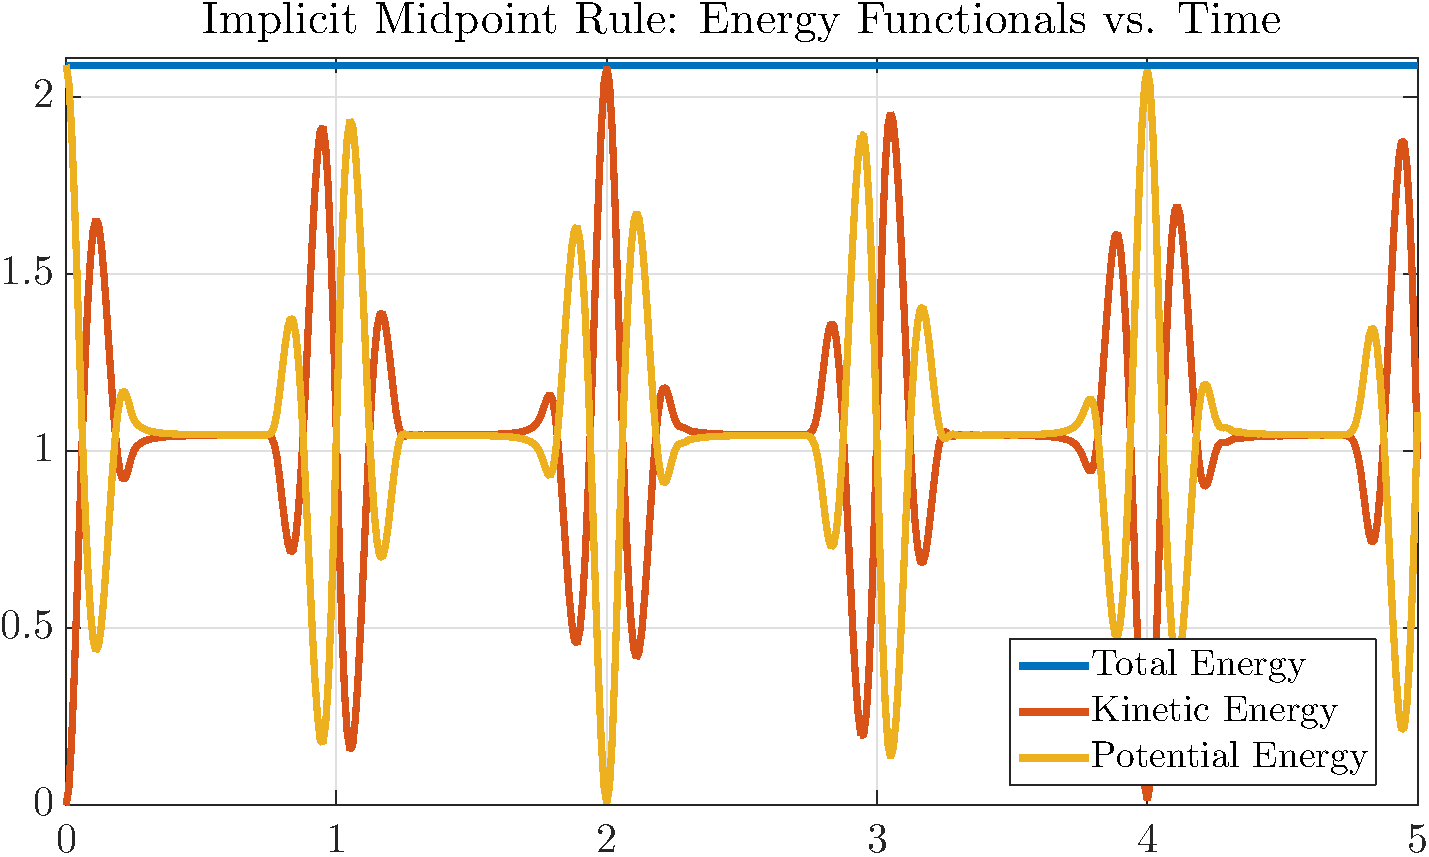
\includegraphics[width=6in, height=4in]{../fenics/cn.pdf}
\captionof{figure}{Plots of the total energy, kinetic energy, and potential energy obtained when solving the homogenous wave equation using the implicit midpoint rule.
Note the conservation of energy throughout time.\label{fig:cn}}
\vfill
\newpage
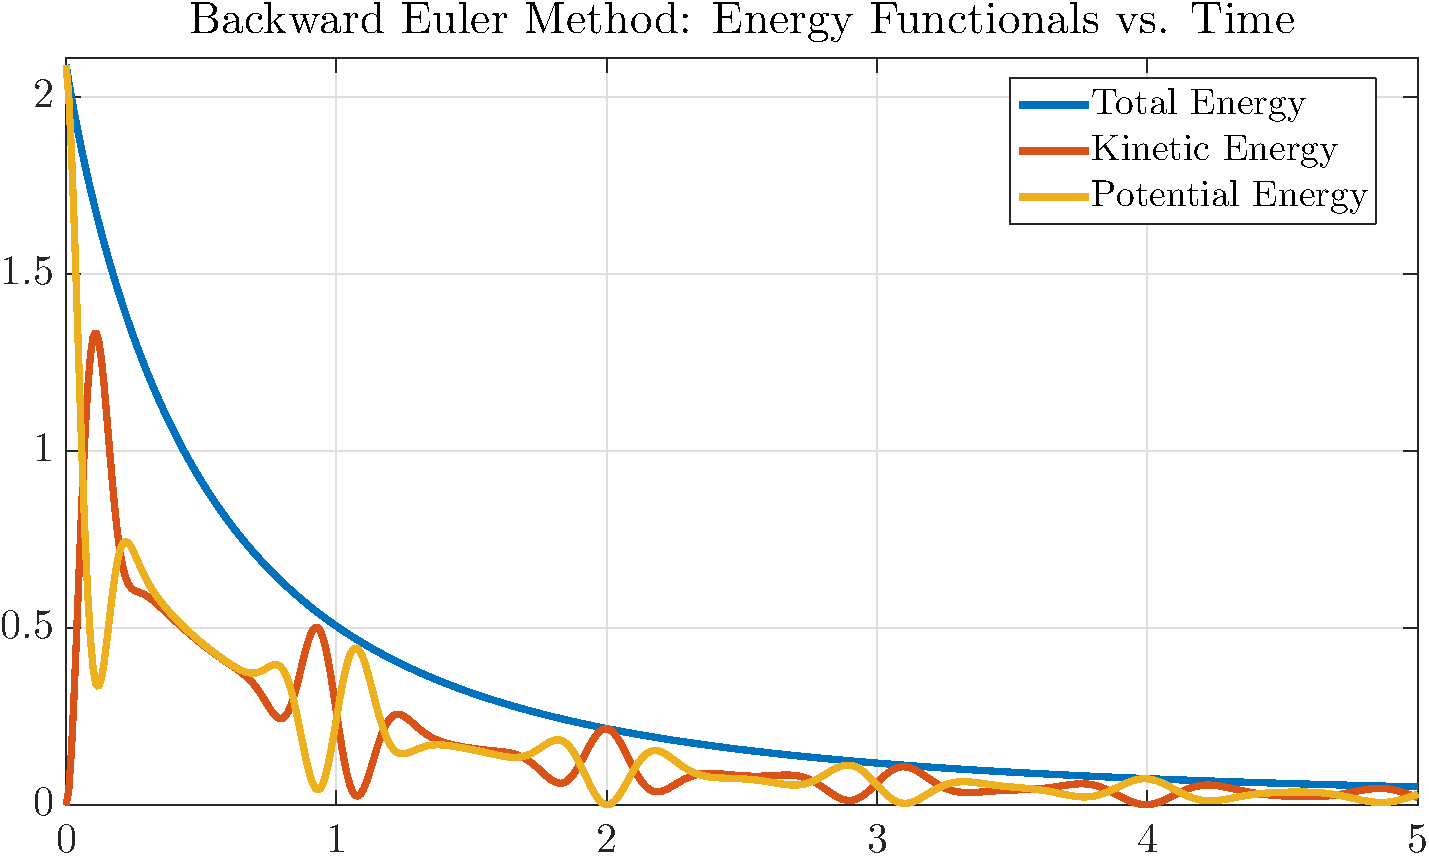
\includegraphics[width=6in, height=4in]{../fenics/be.pdf}
\captionof{figure}{Plots of the total energy, kinetic energy, and potential energy obtained when solving the homogenous wave equation using the backward Euler method.
Note the exponential decay of the total energy throughout time.\label{fig:be}}
\vfill
\newpage
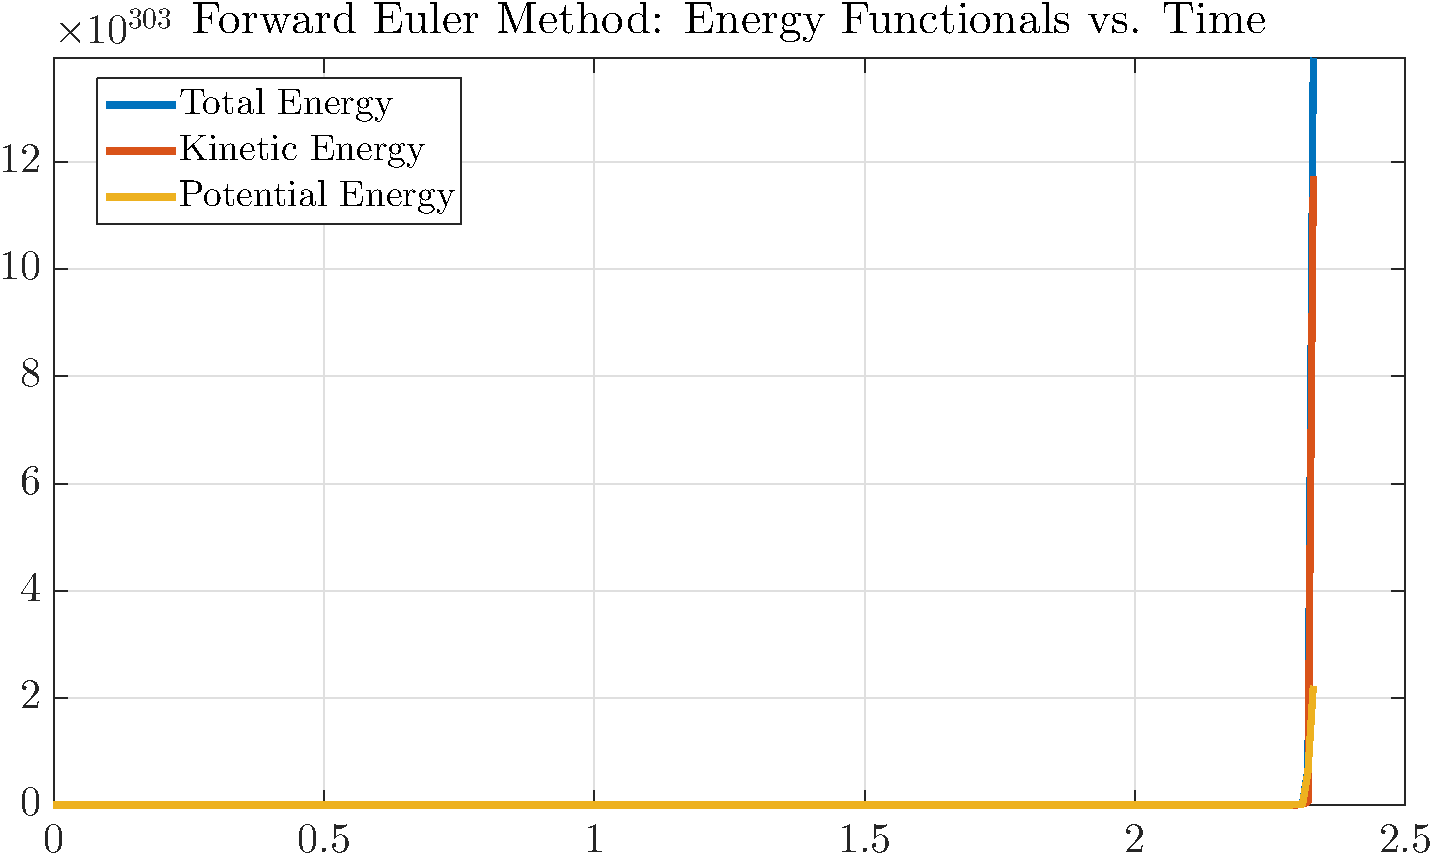
\includegraphics[width=6in, height=4in]{../fenics/fe.pdf}
\captionof{figure}{Plots of the total energy, kinetic energy, and potential energy obtained when solving the homogenous wave equation using the forward Euler method.
Note the exponential blowup of the solution due to the instability of the method.\label{fig:fe}}
\vfill\null
}

% ------------------------------------------------------------ %
% Appendix 2: Code
% ------------------------------------------------------------ %
\newpage
\lhead{}
\section{}\label{hw10Code}
\textbf{\Large\code{hw10.py}}
\includecode{../fenics/hw10.py}

\newpage
\textbf{\Large\code{energyplots.m}}
\includecode{../fenics/energyplots.m}

\end{appendices}


\end{document}
